\section{The Multicast Protocol}

\subsection{Memory management}

\begin{figure}[ht!]
  \centering
  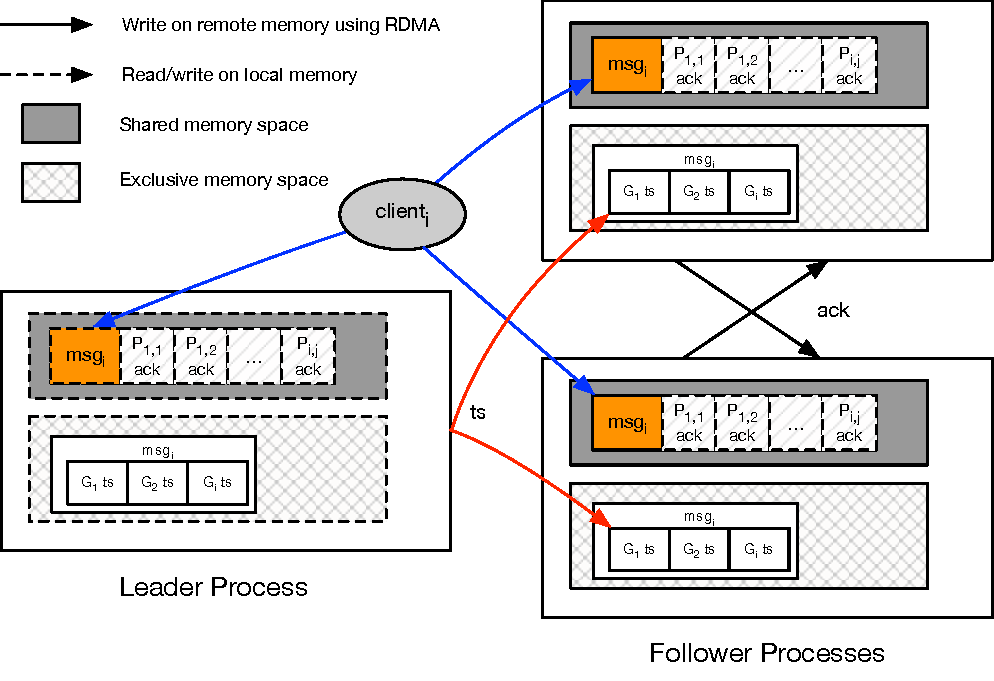
\includegraphics[width=1\linewidth]{figures/memory}
  \caption{Memory layout of \proto. Each process has shared and exclusive memory
  space. All other processes can access shared memory. Only leader can access
  exclusive memory }
  \label{fig:normal_operation_time}
\end{figure}

Each process of \proto organizes its memory with two memory regions: shared
memory and exclusive memory spaces. All processes have remote access
(read/write) to the shared memory space. Only one process (leader) of each group
has has remote-write permission to a given node’s log at any point in time
during the protocol.

The shared memory space is a circular buffer of fixed-size entries with a
sequential index. Client keep a copy of the remote head and tail pointer. Client
increase remote tail after writing to the shared memory. Server process update
the head pointer on client after delivering message by piggying back the new
value in the response.

Each process $p$ periodically polls the memory cell at Head position of each
connected QPs to detect new message.

For each message $m$ written in the shared memory, there is a corresponding cell
in the exclusive memory space reserved for timestamps of $m$

\subsection{Normal case}

\begin{figure}[ht!]
  \centering
  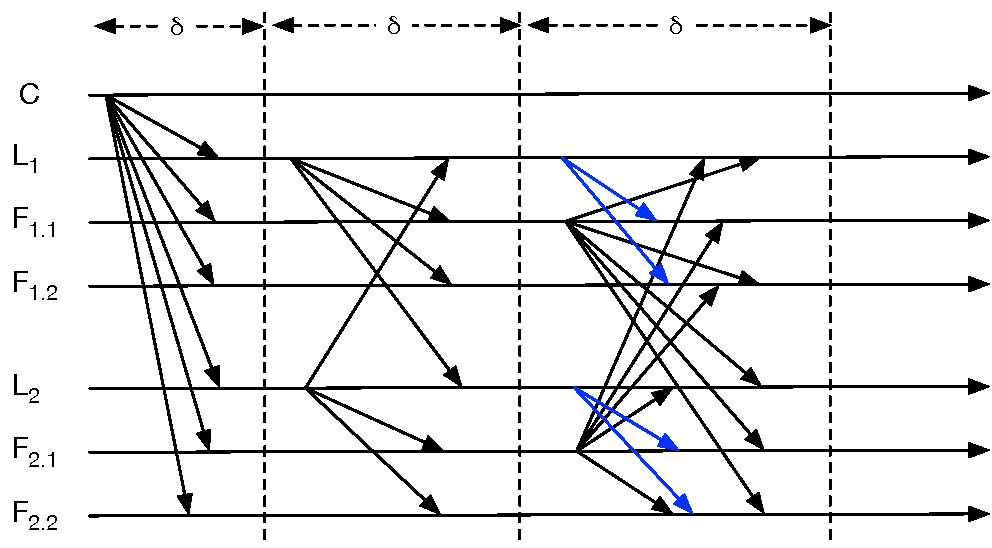
\includegraphics[width=1\linewidth]{figures/timeline-simple}
  \caption{Normal case execution of \proto. Step 1: client writes message to all
          involves processes. Step 2: leader of each group in the destination
          propose and write a timestamp to all followers and other leaders
          memory. Step 3: leaders propagate the timestamp written by other
          leaders, followers write their acks for local timestamp on all other
          processes}
  \label{fig:normal_operation_time}
\end{figure}

%!TEX root =  main.tex
\begin{algorithm*}
\footnotesize

\begin{distribalgo}[1]

\INIT
	\STATE $ts \leftarrow 0$
	\COMMENT{P's logical clock}
	\STATE $pending \leftarrow \emptyset$
	\COMMENT{set of message to be ordered}
	\STATE $ordered \leftarrow \emptyset$
	\COMMENT{set of message already ordered, to be delivered}
	\STATE $pending_{ts} \leftarrow \emptyset$
	\COMMENT{set of pending slots for timestamps}
	% \STATE $pending_{ack} \leftarrow \emptyset$
	% \COMMENT{set of pending slots for acknowledgements}
	\STATE $bal \leftarrow 0$
	\COMMENT{ballot number}
	\STATE $seq \leftarrow 0$
	\COMMENT{sequence number}
	\STATE $curSeq \leftarrow 0$
	\COMMENT{P's current sequence number}
	\STATE $\buffer \leftarrow NULL$
	\COMMENT{P's local buffer}
	\vspace{2.0mm}
\ENDINIT
\vspace{2.0mm}

\INDENT{\colorbox{\coloralgo}{to a-mcast message m	:}}
	\FORALL[\textbf{Task 1}] {$p \in G \mid \forall G \in  m.dest$}
		\TRIGGER {$ \langle rdma, \WRITE \mid p, [m] \rangle$}
		\COMMENT{remote-write m to memory of all processes belong to all involved groups}
	\ENDFOR
\ENDINDENT
\vspace{2.0mm}

\INDENT{\colorbox{\coloralgo}{leader process $P_L$ of group $G$}}
	\UPON[\textbf{Task 2} on receive message $m$ in local buffer]{$\langle \buffer, \READ \mid m \rangle$}
		\STATE $dest \leftarrow \{\forall p \mid p \in G\} \cup \{\forall p \in G_i \mid G_i \in m.dest \wedge p.isLeader\}$
		\COMMENT{set of all processes in G and all leaders of involved groups}
		\STATE $ts \leftarrow ts + 1$
		\COMMENT{increase local timestamp}
		\STATE $seq \leftarrow seq + 1$
		\COMMENT{increase sequence number}
		\FORALL {$p \in dest$}
			\TRIGGER {$ \langle rdma, \WRITE \mid p, [P_L, bal, seq, ts] \rangle$}
			\COMMENT{remote-write $P_l$'s timestamp with ballot $bal$ and sequence $seq$ to all process $\in dest$ set}
		\ENDFOR
	\ENDUPON
	\vspace{2.0mm}

	\UPON[\textbf{Task 3} on receive timestamp $ts_l$ of a leader $P_l$ in local buffer]{$\langle \buffer, \READ \mid [P_l, bal_l, seq_l, ts_l] \rangle$}
		\STATE $seq \leftarrow seq + 1$
		\COMMENT{increase sequence number}
		\FORALL {$p \in G$}
			\TRIGGER {$ \langle rdma, \WRITE \mid p, [P_l, bal, seq, ts_l] \rangle$}
			\COMMENT{propagate $P_l$'s timestamp $ts_l$ with its ballot and sequence number $seq$ to all process $\in dest$ set}
		\ENDFOR
		\STATE $ts \leftarrow max(ts, ts_l)$
	\ENDUPON
\ENDINDENT
\vspace{2.0mm}

\INDENT{\colorbox{\coloralgo}{any process $P$ of group $G$}}
	\UPON[\textbf{Task 4} on receive message $m$ in local buffer]{$\langle \buffer, \READ \mid m \rangle$}
		% \STATE do $\READ(ts, L)$
		\STATE $pending \leftarrow pending \cup \{m\}$
		\COMMENT{include m in pending messages set}
		% \COMMENT{polling timestamp of leader of its own group}
		\STATE $pending_{ts} \leftarrow pending_{ts} \cup \{\langle m_{id}, G \rangle \mid \forall G, G \in m.dest \}$
	\ENDUPON
	\vspace{2.0mm}

	\WHEN{true}
		\IF[\textbf{Task 5} ]{$ \exists \langle m_{id}, G \rangle \in pending_{ts} : ts_G \neq 0 $}
			\STATE $ts \leftarrow max(ts, ts_G)$
            		\COMMENT{Lamport’s rule to update logical clocks}
            		\FORALL {$p \in m.dest$}
            			\TRIGGER {$ \langle rdma, \WRITE \mid p, [P, ack] \rangle$}
            			\COMMENT{remote-write P's ack to memory of all involved processes}
            		\ENDFOR

			% \STATE $pending_{ack} \leftarrow pending_{ack}$ \textbackslash $\{ \langle m_{id}, G \rangle \}$
            		\STATE $pending_{ts} \leftarrow pending_{ts} \cup \{ \langle m_{id}, G, c_w \rangle \}$
            		\COMMENT{include $\langle ts_l, c_w, m \rangle$ in pending timestamps set}

			\WHILE[refer to note]{$\exists \langle m_{id}, G, c_w \rangle \in pending_{ts} : c_w = curSeq + 1$}
            			\STATE $pending_{ts} \leftarrow pending_{ts}$ \textbackslash $\{\langle m_{id}, G \rangle\}$
            			\COMMENT{remove $\langle m_{id}, G \rangle$ from ts pending set}
            			\STATE  $curSeq = curSeq + 1$
            			\COMMENT{increase current sequence number}
            		\ENDWHILE

            		\WHILE[]{$\exists m \in pending : isFulfilled(m) = true$}
            			\STATE $t \leftarrow max(ts_i)$
            			\COMMENT{$t$ is the largest timestamp between all timestamps $ts_i$ populated by all leaders}
            			\STATE $pending \leftarrow pending$ \textbackslash $\{m\}$
            			\COMMENT{remove $m$ from pending set}
            			\STATE $ordered \leftarrow ordered \cup \langle m, t \rangle$
            			\COMMENT{include $\langle m, t \rangle$ in ordered set}
            		\ENDWHILE

            		% \WHILE {$\exists \langle m,t \rangle \in ordered : t < min(\forall t_i \in pending) \wedge \newline
            		% 		\hspace*{11.7em} t < min(\forall t_i \in ordered)$:}
            		\WHILE {$\exists \langle m,t \rangle \in ordered : t < min(\forall t_i \in pending) \wedge t < min(\forall t_i \in ordered)$:}
            			\STATE $ordered \leftarrow ordered$ \textbackslash $\{m\}$
            			\STATE deliver $m$
            		\ENDWHILE
		\ENDIF
	\ENDWHEN
\ENDINDENT
\vspace{4.0mm}

% \INDENT{\colorbox{\coloralgo}{\textbf{function} \rwrite$(dest, data\dots)$}}
% 	\STATE rdma-write $[data\dots]$ to $dest$'s shared buffer
% \ENDINDENT
% \vspace{2.0mm}

% \INDENT{\colorbox{\coloralgo}{\textbf{function} \READ$(data\dots)$}}
% \STATE atomic-read $[data\dots]$ from local buffer
% \ENDINDENT
% \vspace{2.0mm}

\INDENT{\colorbox{\coloralgo}{\textbf{function} isFulfilled$(m)$}}
	\IF[m receives ts of all involved groups and acks from majority processes]{$\forall G \mid G \in m.dst \wedge \newline
	\hspace*{3.5em} ts_G \neq 0 \wedge \newline
	\hspace*{3.5em} \langle m_{id}, G, c_w \rangle \notin pending_{ts} \wedge \newline
	\hspace*{3.5em} $ received acks for $ts_G$ from majority:}
		\RETURN true
	\ELSE
		\RETURN false
	\ENDIF
\ENDINDENT

\caption{Normal case execution}
\label{alg:normal_case}
\end{distribalgo}
\end{algorithm*}


The normal operation protocol is involved when there is an existence of a sole
leader per group that has the support of at least a majority of processes of
that group. A leader is responsible for proposing timestamp for new message, and
propagating timestamps from other groups to followers of its local group.

A client process $C$ multicasts a message $m$ to a set of target groups in
$m.dst$ by performing a \rwrite to the same memory entry on the shared memory of
each process $p_i$ belongs to $m.dst$. (Task 1 algorithm~\ref{alg:normal_case})

Once leader process $L$ in group $g$ \lread the message $m$, it computes a
group-wise timestamp $ts$ and writes that proposed timestamp $ts$ to the memory
cell reserved for $m$ in the exclusive memory space of: (1) all follower
processes $f$ belongs to $g$. (2) all leader processes $L_i$ of other groups
$g_i$ belongs to $m.dst$ The proposed timestamp $ts$ consists of three
components: the ballot number $bal$ in which $L$ is the leader of group $g$, the
sequence number $sel$ is the consensus instance of message $m$ in group $g$, and
$v$ is $L$'s logical clock value. (Task 2 algorithm~\ref{alg:normal_case})

Upon \lread a timestamp $ts$ of message $m$ from leader processes of other
groups, a leader $L$ propagates that timestamp to its group by performing
\rwrite $ts$ to the exclusive memory space for $m$ in all follower processes of
its local group. (Task 3 algorithm~\ref{alg:normal_case})

Once each involved process $P$ belongs to $m.dst$ \lread message $m$ in its
local buffer, $P$ mark the message as pending, and starts polling from it
exclusive memory for timestamps of $m$ (Task 4 algorithm~\ref{alg:normal_case}).

Upon \lread a timestamp $ts$ of message $m$ from leader of local group, a
process $P$ writes its acknowledgement $ack$ for that timestamp to the shared
memory of all other involved processes, and start polling from its memory for
acknowledgements from other processes. (Task 4 algorithm~\ref{alg:normal_case}).
Once $P$ receives timestamps of all involved groups and acknowledgements from
the majority of processes of each group, it can order the message $m$ and starts
deliver it.

\subsection{Leader election}

\proto assumes the existence of an unreliable failure detector. If a leader is
slow or crashes, the failure detector will detect this and elect new leader.
When a process becomes a leader, it needs to perform several steps to ensure it
is the only leader of its groups. Those steps are: (1) increasing ballot number,
in which that process becomes leader. (2) sending 1A message to all processes
with new ballot number, and wait for the response of majority (3) ensure the
logs of all processes are up-to-date

Firstly, the new leader must choose a new ballot number that is higher than all
ballot numbers before. A process only reply to the message or timestamp that has
a ballot number higher than its current value. The new ballot number will be
included in each timestamp $ts$ of this leader later.

Then the new leader needs to get the access to the exclusive memory space on (1)
the followers of its local group, and (2) the leaders of other groups. In order
to act as a leader, a node must get the write permission from majority of other
processes in its group. In addition, to tolerate failure of the leaders of other
groups, the new leader also need to get the write permission from majority of
processes of other groups. The new leader request the access by issuing a RDMA
Send (\lle{this could be a \rwrite}) that includes a new ballot number, the
sequence number of the most recent deliver message. When a process receives this
message, it checks if the ballot number is higher than its current ballot value,
then revokes access of the old leader, and send a reply to the new leader with
its current sequence number

Finally, once the new leader receives reply from majority processes, it must
ensure all remote logs are up-to-date with its own. If the sequence number of
leader is smaller than follower, the leader should know that for missing
instances, it can read the agreed timestamps from followers.

With the pending instances (the instances in the pending list without
timestamps, or has not received majority of acks), leader can just rewrite new
timestamp value with its new ballot number. In this case leader issues a RDMA
WRITE-WITH-IMM which triggers a completion event at the receivers side.



% not necessary
% if the sequence number of leader is bigger than follower, the follower can do a
% \rread of missing timestamps from leader's memory.
